% This text is proprietary.
% It's a part of presentation made by myself.
% It may not used commercial.
% The noncommercial use such as private and study is free
% Nov. 2006
% Author: Sascha Frank 
% University Freiburg 
% www.informatik.uni-freiburg.de/~frank/
%
% additional usepackage{beamerthemeshadow} is used
%  
%  \beamersetuncovermixins{\opaqueness<1>{25}}{\opaqueness<2->{15}}
%  with this the elements which were coming soon were only hinted
\documentclass{beamer}
%\usepackage{beamerthemesplit}
\usepackage{asymptote}
\usepackage[update,prepend]{epstopdf}
\usepackage{subfigure}
%\usepackage{cite}
%\usepackage[cmex10]{amsmath}
\usepackage{amsfonts}
\usepackage{url}
\usepackage{pgf}
\usepackage{tikz}
\usetikzlibrary{arrows,chains,matrix,positioning,scopes}
%
\makeatletter
\tikzset{join/.code=\tikzset{after node path={%
\ifx\tikzchainprevious\pgfutil@empty\else(\tikzchainprevious)%
edge[every join]#1(\tikzchaincurrent)\fi}}}
\makeatother
%
\tikzset{>=stealth',every on chain/.append style={join},
         every join/.style={->}}
\tikzstyle{labeled}=[execute at begin node=$\scriptstyle,
   execute at end node=$]
\usepackage[style=ieee]{biblatex}
\addbibresource{presentation}
%\ExecuteBibliographyOptions{numeric-comp}

\def\docversion{Notes Version 0.1}

\usetheme{Luebeck}
\usecolortheme{lily}
\usefonttheme{serif}
\title{Sensors for FRC}  
\author{Dr. Travis W. Axtell \\ \emph{travis.axtell@gmail.com}}
\institute{Mentor for FRC Team 612 --- Chantilly, VA \\ 
\quad\quad\quad\, FRC Team 
2035 --- 
Carmel, CA \\ \quad\quad\quad\quad\quad\quad FRC Team 5104 --- Pacific Grove, 
CA}
\date{\docversion\\ \today} 

\addtobeamertemplate{footnote}{}{\vspace{2ex}}

\setbeamercolor{block title}{use=structure,fg=white,bg=blue!75!black}
\setbeamercolor{block body}{use=structure,fg=black,bg=black!20!white}
\setbeamertemplate{blocks}[rounded][shadow=true]
%\setbeamertemplate{blocks}

\begin{document}

\frame{\titlepage} 

\frame{\frametitle{Table of contents}\tableofcontents} 


\section{Introduction} 
\frame{ 
\frametitle{How to read these notes}
\begin{itemize}
\item Underlined terms are concepts you should strive to understand, with the 
goal of being able to explain the concepts to others.
\item Investigate the meaning of new math notation.  Wikipedia can help --- see 
\url{https://en.wikipedia.org/wiki/List_of_mathematical_symbols}.
\item I am available for discussions when you need help.
\end{itemize}
}

\subsection{Definitions}
\frame{\frametitle{Definitions}
A \underline{Transducer}:  
\\
A continuous signal
A discrete signal
}

\frame{\frametitle{Definitions}
A \underline{analog signal}:
\\
A \underline{digital signal}:  
\\
A \underline{pulse-width modulated} (PWM) signal:
\\
An \underline{input} signal is a signal generated on some external hardware 
that is going into the RobotRIO.
\\
An \underline{output} signal is a signal generated on the RobotRIO that is 
going to external hardware.
}

\frame{\frametitle{Definitions}
Noise is random changes to the signal due to physical properties of the sensor.
All sensors are subject to noise.  Noise can only be quantified by statistics, 
as its actual value $n(t)$ cannot be known.

It is desirable for a control system to be \underline{Robust} to noise, meaning 
that the noise does not strongly affect the output.

\underline{Uncertainty} is the incorrect (or absent) modeling of a system.

}


\subsection{Hardware}
\frame{
\frametitle{RobotRIO}
\includegraphics[width=\textwidth]{RobotRio}
}

\frame{
\frametitle{Old hardware}
\includegraphics[width=2in]{DigitalSideCar}
\includegraphics[width=2in]{AnalogSideCar}
}

\section{Sensors}
\subsection{Simple}
\frame{
\frametitle{Contact switch}
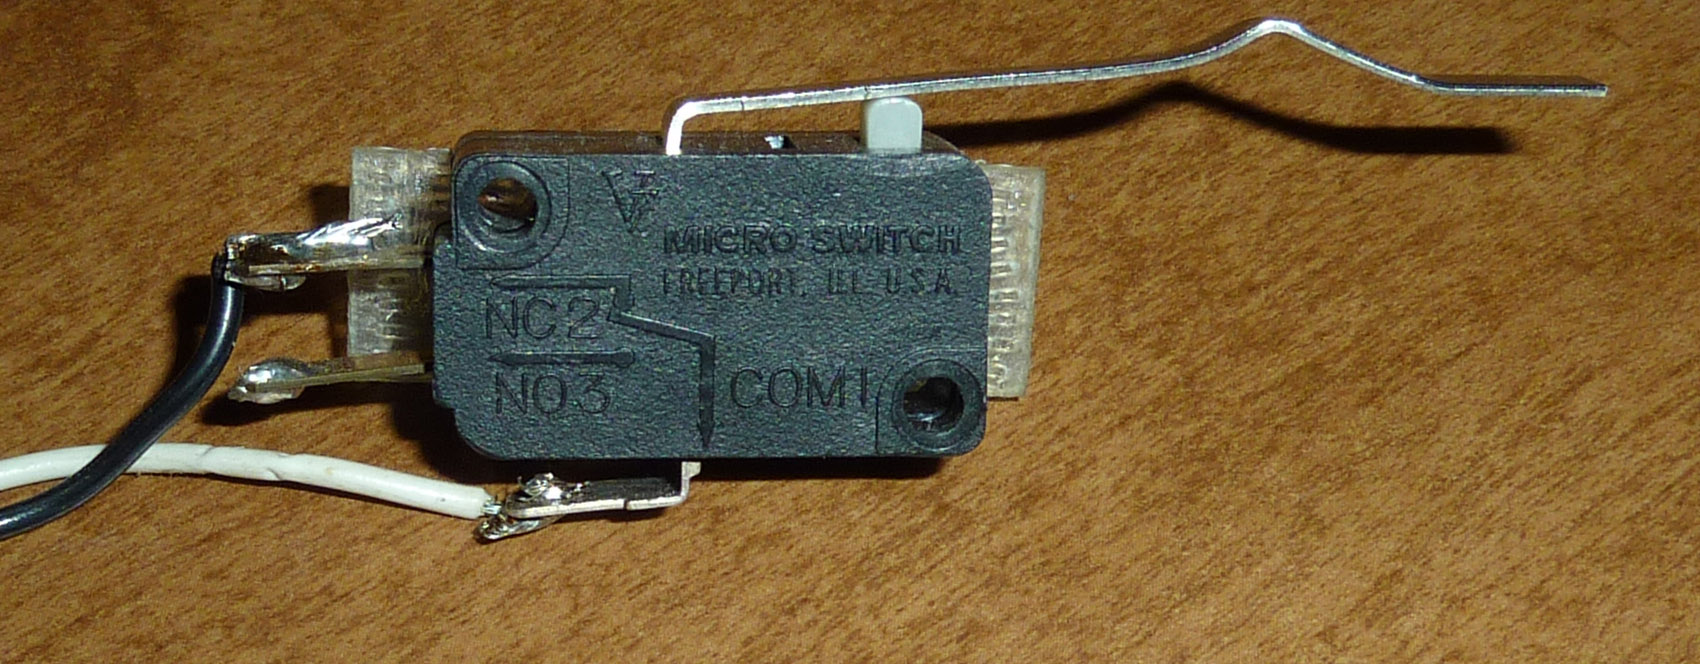
\includegraphics[width=\textwidth]{LimitSwitch}
}

\frame{
\frametitle{Electronic switch}
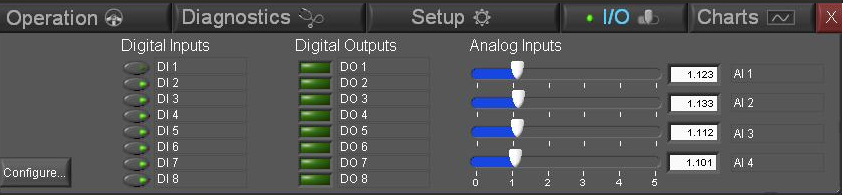
\includegraphics[width=\textwidth]{DriverStation}
}

\frame{
\frametitle{Potentiometer}
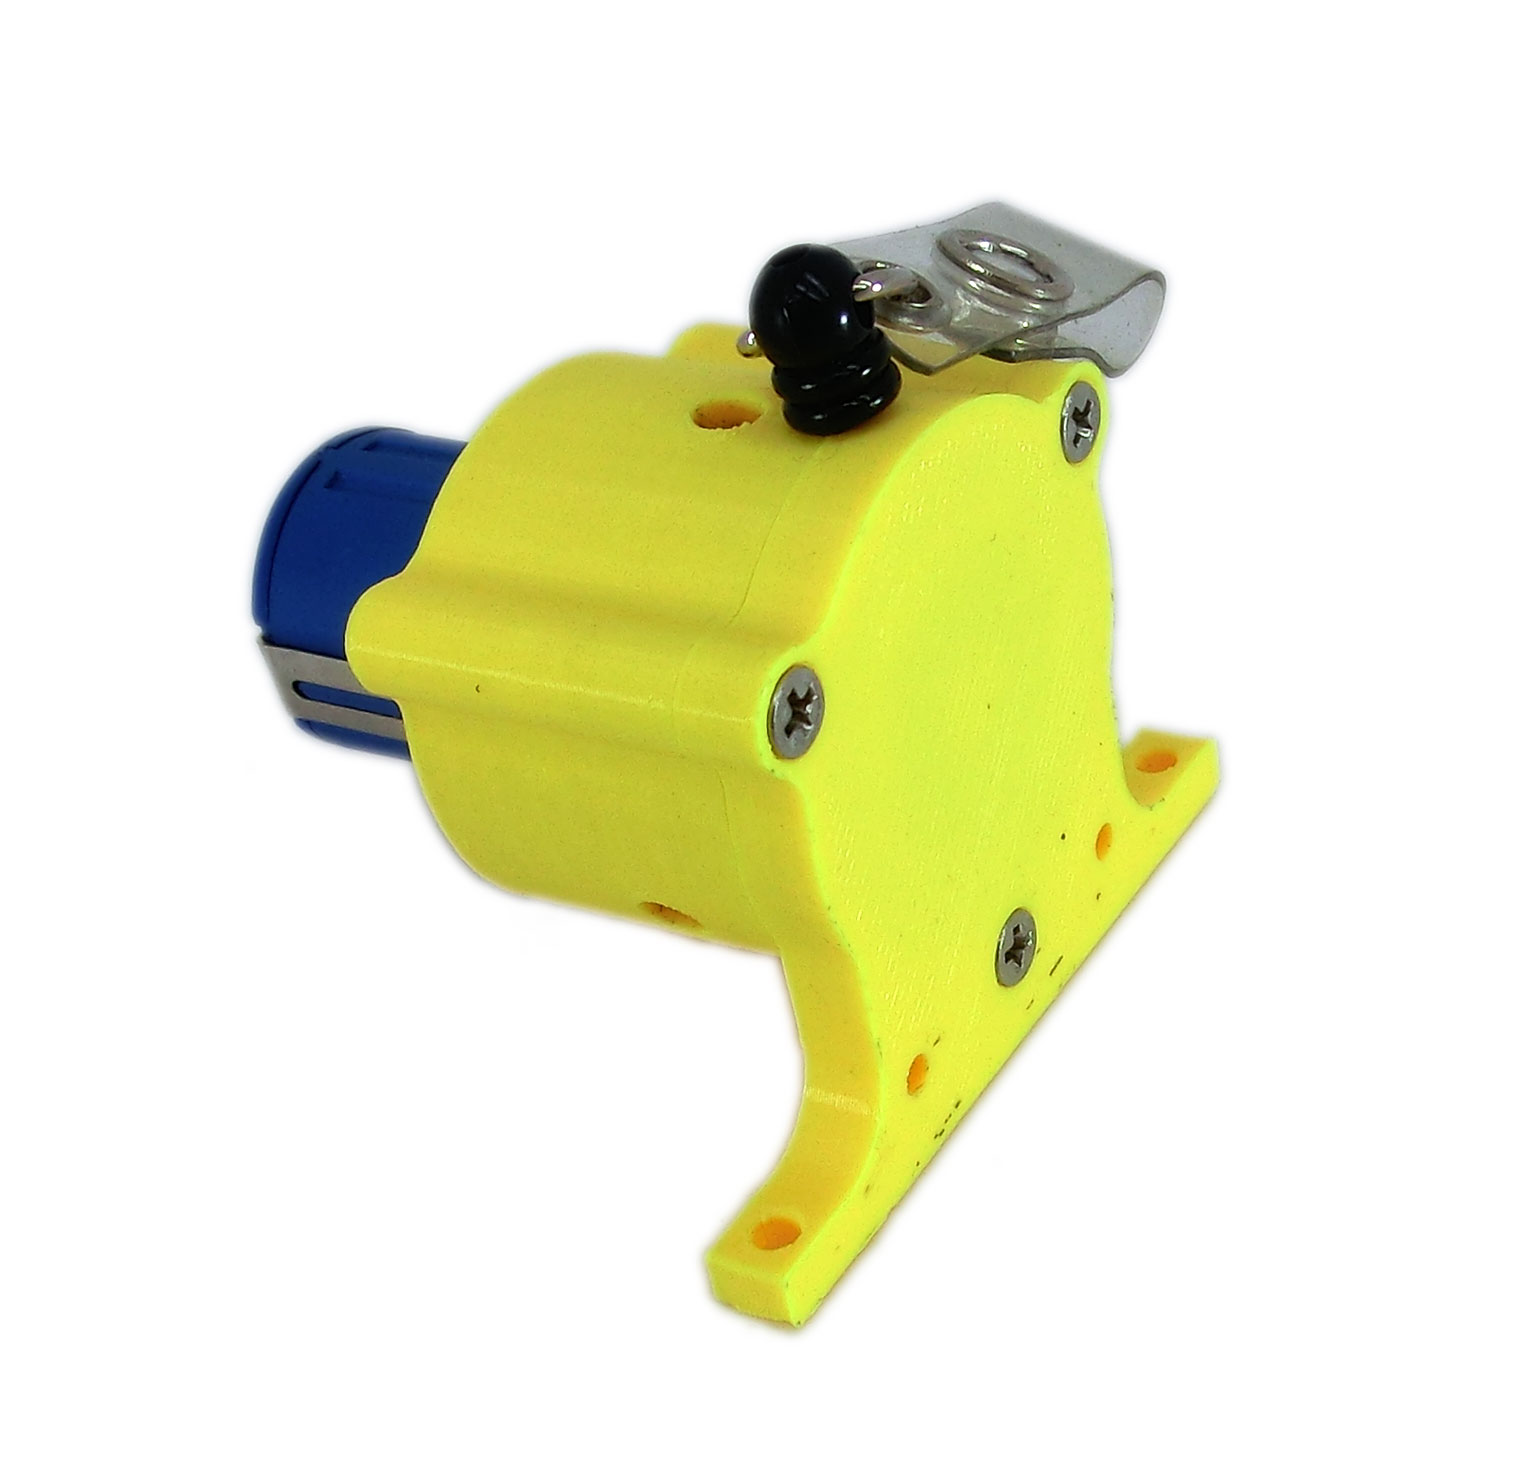
\includegraphics[width=1in]{Potentiometer}
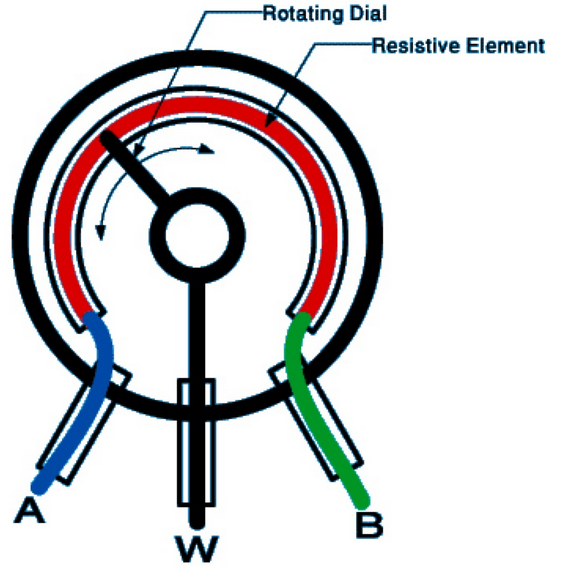
\includegraphics[width=1in]{Potentiometer2}
}

\frame{
\frametitle{Rotary encoder}
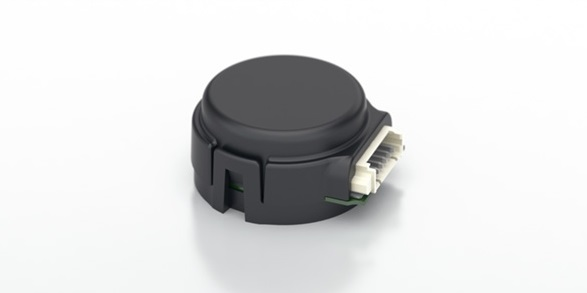
\includegraphics[width=1in]{OpticalEncoder}
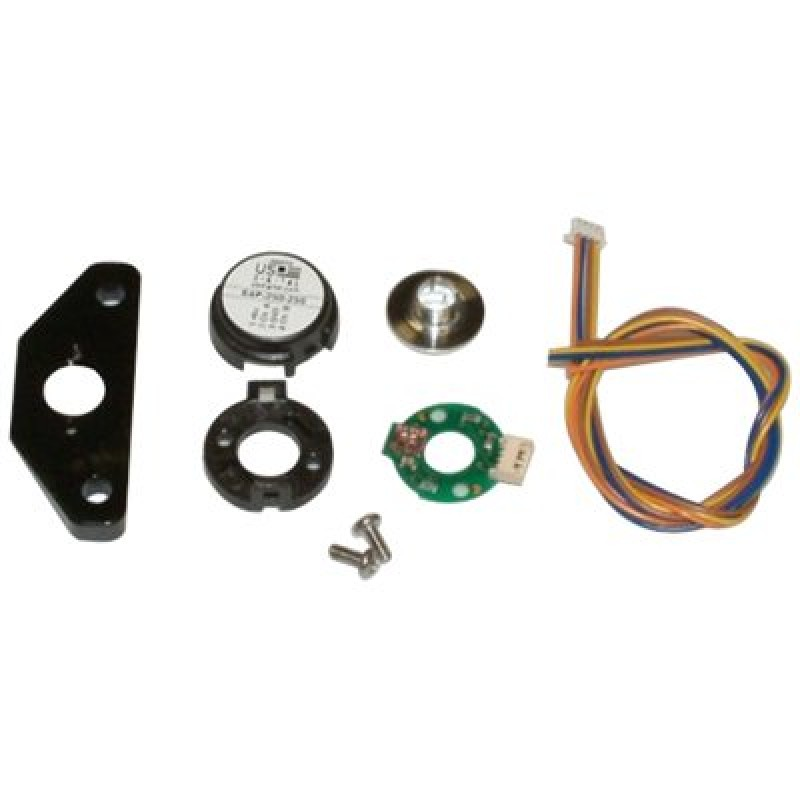
\includegraphics[width=1in]{OpticalEncoder2}
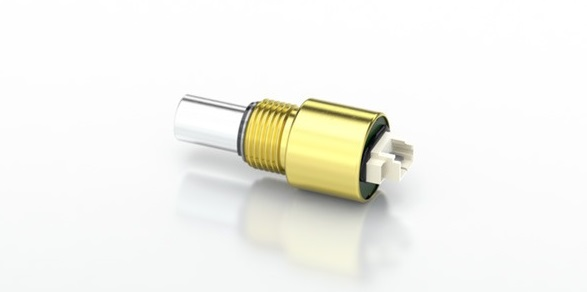
\includegraphics[width=1in]{MagneticEncoder}
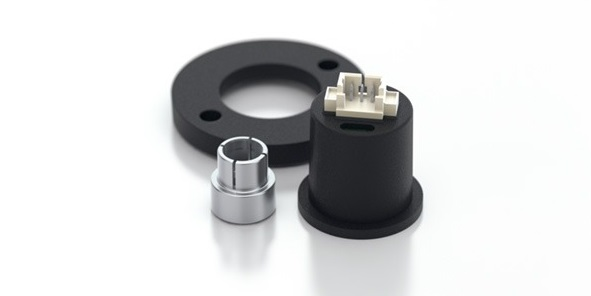
\includegraphics[width=1in]{MagneticEncoder2}
}

\subsection{Imaging}
\frame{
\frametitle{AXIS Webcam}
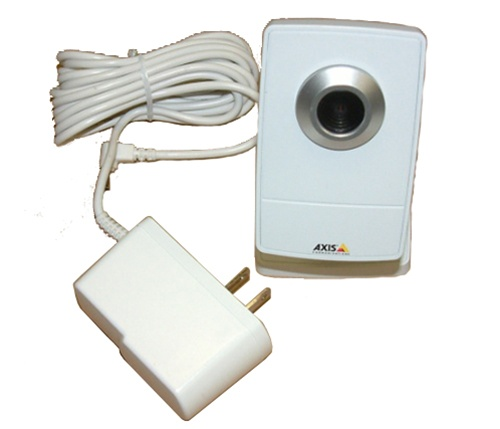
\includegraphics[width=1in]{AXISwebcam}
}

\frame{
\frametitle{PixyCam}
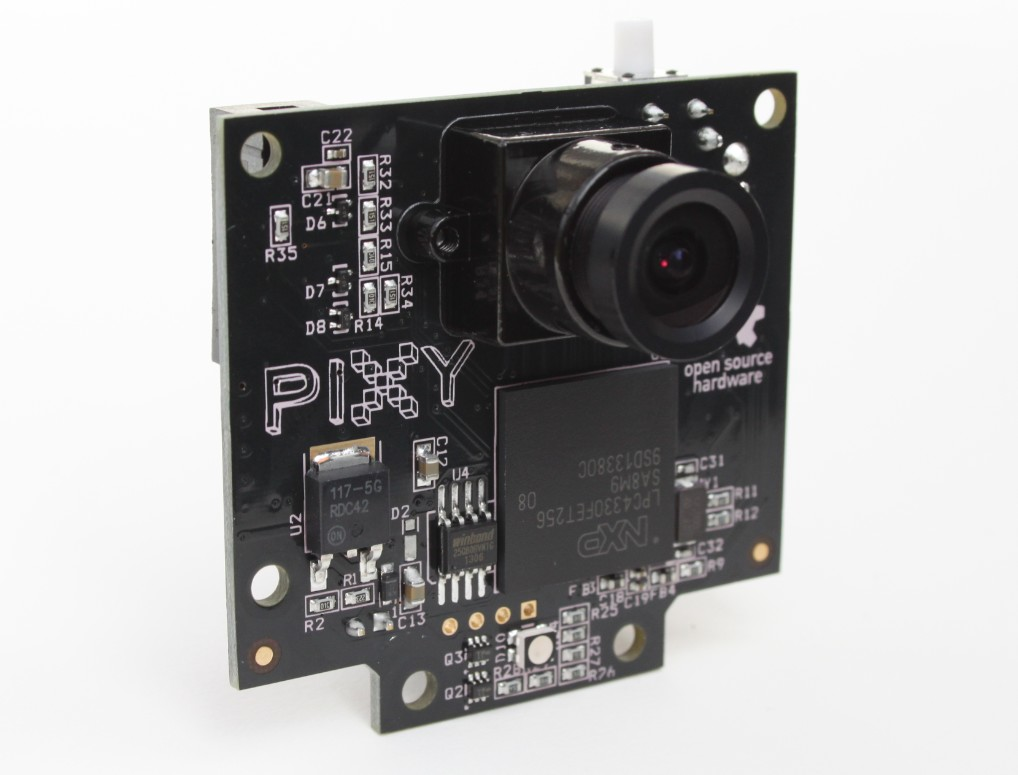
\includegraphics[width=1in]{PixyCam}
}

\frame{
\frametitle{Kinect}
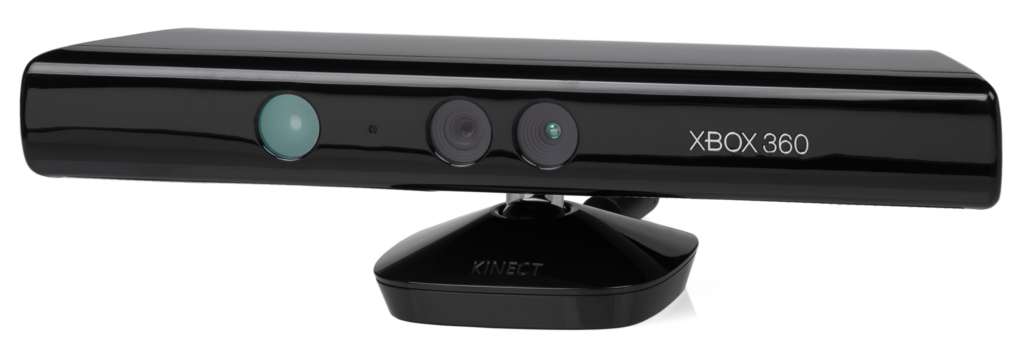
\includegraphics[width=\textwidth]{kinect}
}

\frame{
\frametitle{Kinect}
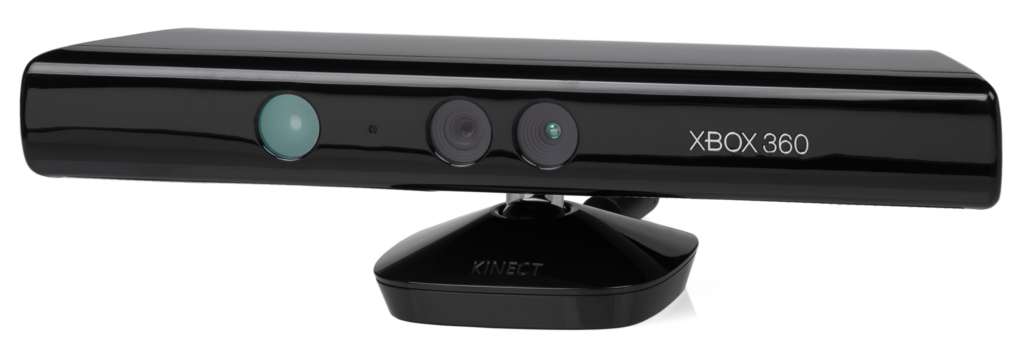
\includegraphics[width=1in]{kinect}
}

\frame{
\frametitle{Playstation Camera}
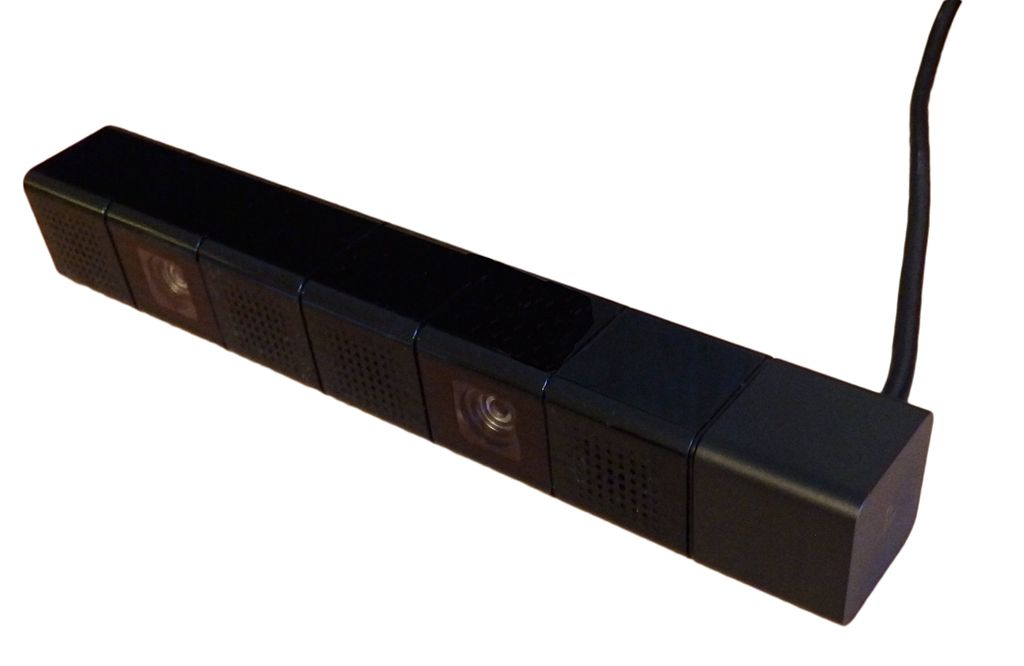
\includegraphics[width=1in]{PlaystationCamera}
}

\subsection{Location and Orientation}
\frame{
\frametitle{Gyro}
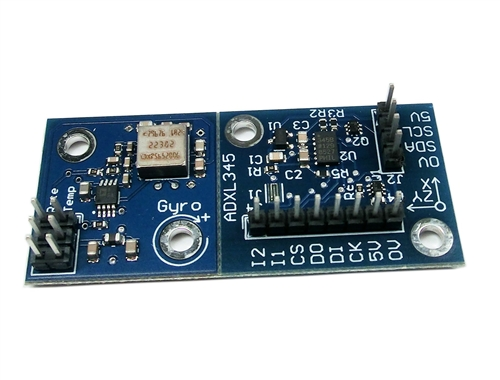
\includegraphics[width=1in]{Gyro}
}

\frame{
\frametitle{Accelerometer}
}

\frame{
\frametitle{GPS}
}

\frame{
\frametitle{Indoor GPS}
}

\subsection{Distance estimation}
\frame{
\frametitle{Ultrasonic rangefinder}
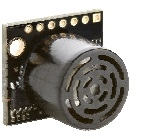
\includegraphics[width=1in]{Ultrasonic}
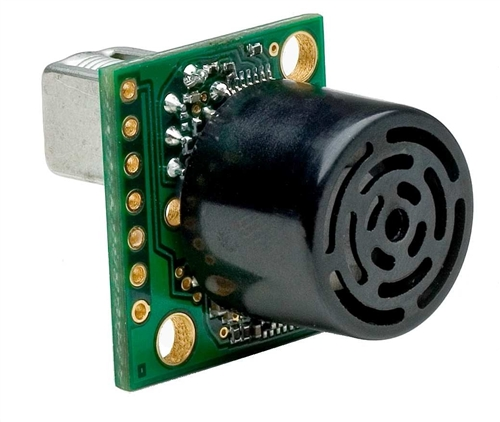
\includegraphics[width=1in]{Ultrasonic2}
}

\frame{
\frametitle{Laser rangefinder}
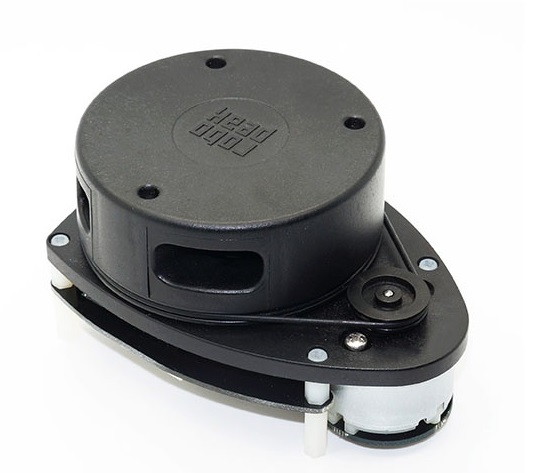
\includegraphics[width=1in]{LaserRangefinder}
}

\section{Haptic and Controls}
\frame{
\frametitle{Vibrating joystick}
}

\frame{
\frametitle{Wii controller Wiimote}
}

\frame{
\frametitle{Wii balance board}
}

\section{Conclusion}
\frame{
\frametitle{LEGO Mindstorm}
The LEGO Mindstorm has equivalent sensors for:
Color, light detection, axis rotation, contact, IR, ultrasonic, ...
}

\subsection{Resources}
\frame{ 
\frametitle{Resources}
[1] \href{http://www}{\underline{TBD}}
}

\end{document}
